\documentclass{article}
\usepackage{afterpage}
\usepackage[a4paper,bindingoffset=0.2in,
            left=1.1in,right=1.1in,top=1.1in,bottom=1.1in,
            footskip=.25in]{geometry}
\usepackage{pdfpages}
\usepackage{indentfirst}

\newcommand\blankpage{%
    \null
    \thispagestyle{empty}%
    \addtocounter{page}{-1}%
    \newpage}

\begin{document}

\afterpage{\blankpage}

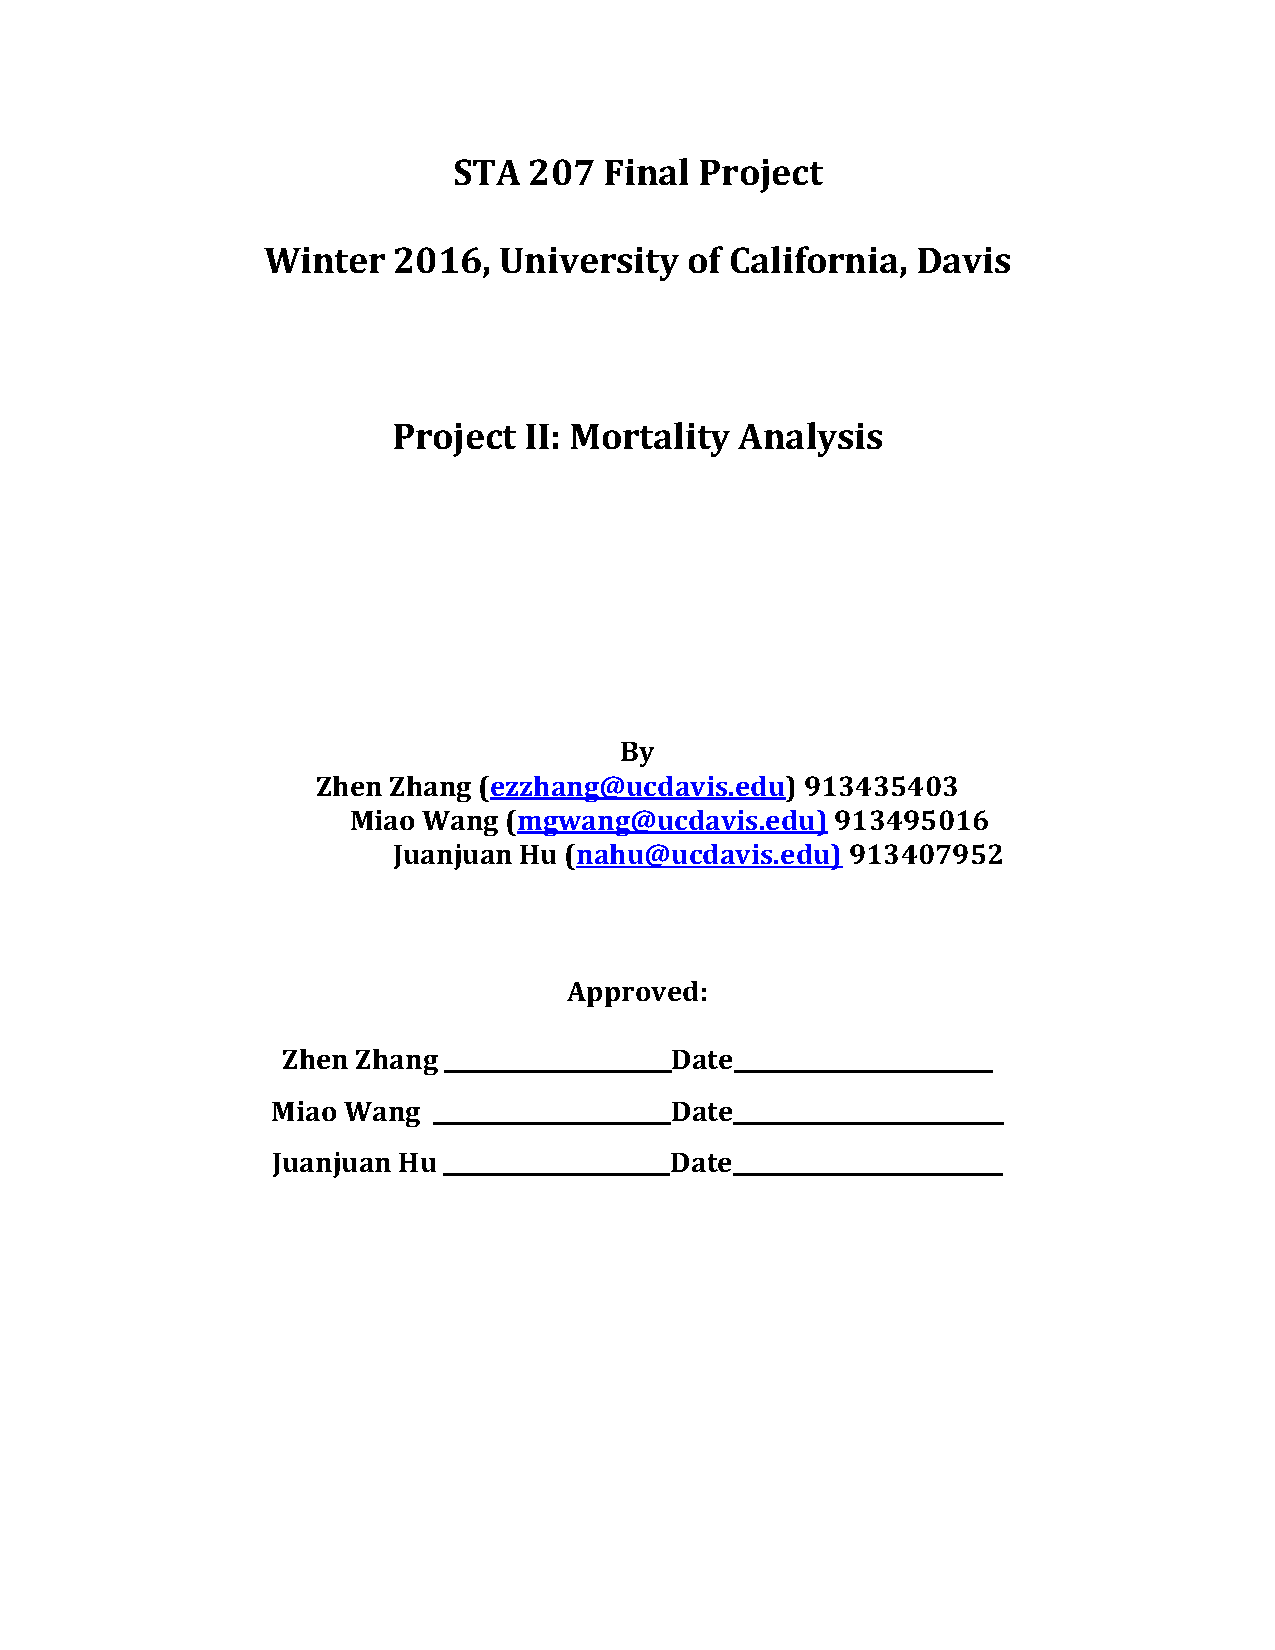
\includepdf[pages=-,pagecommand={\thispagestyle{plain}}]{STA207_project_cover.pdf}

\setcounter{page}{1}

\section{Introduction}
   Interests in identifying factors that have associations with human mortality arise from their importance in better understanding causes to mortality and in helping people improve their life quality. Many researchers work on studying relationships between mortality and various factors including weather, smoking, social relationship, etc.
   In our project, we sought to explore associations between mortality with some measures of climate and demography as well as pollution measures. We also discussed in details how the pollution alone affects mortality.

\section{Methods and Results}

  \subsection{Data Description and Exploration}

    \subsubsection{Data Description}

       This dataset contains seven numeric variable: mean annual precipitation (“PRECIP”), median number of school years completed by persons of age 25 or over (“EDUC”), percentage of population in 1960 that is nonwhite (“NONWHITE”), percentage of households with annual income under \$3000 in 1960 (“POOR”), relative pollution potential of oxides of nitrogen (“NOX”), relative pollution potential of sulphur dioxide (“SO2”) and total age-adjusted mortality from all causes (“MORT”). Among these variables, mortality is the response variable and the other six are independent variables. The dataset also contains a column “CITY”, which is a factor variable. Since the number of its levels is the same as the data size (60), it would contribute nothing to explain the mortality in our models. Therefore, we dropped this column.

    \subsubsection{Initial data analysis}
       In order to explore the data, we firstly calculated the summary statistics for all the variables including mean, median and some other important quantiles (Table I.1.2.1). We also constructed each distribution plot (Figure I.1.2.1) and performed simple linear regression for each independent variable (Table I.1.2.2).

    \subsubsection{Transformations and Standardization}
       Based on the distribution plots, we found all the independent variables showed some skewness. Therefore, we did three types of transformation (log, square root, square) for each of them and plot the new distribution plots (Figure I.1.3.1). It turned out that square root transformation is preferred for “NONWHITE” and log transformation is preferred for “POOR” and “SO2”. We also standardized response variables and independent variables so that they are all equally scaled. From now on, all the variables we mention are the transformed and standardized ones.

    \subsubsection{Correlations and Multicollinearity}
       From the correlation matrix (Table I.1.3.1) and the matrix plot (Figure I.1.3.2), we observed correlation present between variables (for example, SO2 and NOX has correlations of 0.7328). Then we calculated the VIF value for each independent variable (Table I.1.3.2) and found that all the VIF are between 2 and 5, indicating moderate multicollinearity among independent variables.

  \subsection{Model Building}

    Here are the results for all the models:

    \begin{center}
         \begin{tabular}{c c c c c c c}
           \hline
           & PRECIP & EDUC & NONWHITE & POOR & NOX & SO2\\
           \hline
           Stepwise & 0.2897 & -0.2024 & 0.4696 & 0.0000 & 0.0000 & 0.3593\\
           PLS      & 0.3738 & -0.2192 & 0.5058 & -0.1251 & 0.1577 & 0.2266\\
           Ridge    & 0.2914 & -0.2122 & 0.3662 & -0.0039 & 0.1454 & 0.2079\\
           Lasso    & 0.2904 & -0.1972 & 0.4160 & 0.0000 & 0.0931 & 0.2535\\
           \hline
         \end{tabular}
       \end{center}

    \subsubsection{Stepwise Regression}
       To deal with multicollinearity among the X variables, we can use stepwise method and AIC criterion to find the best subset of X variables sequentially. In each step, one variable is added or deleted from the model according to AIC.  
       We first considered models with only first order variables. The stepwise procedure ended up with best model (Table II.2.1.1).

       There was a pattern in the residual vs. fitted value plot (Figure II.2.1.1). Some information may be not covered by current model. We considered adding second order variables (including quadratic terms and interaction terms) into the model.  The best model we obtained (Table II.2.1.2) is in the appendix and the residual plot (Figure II.2.1.2) did not improve much.
          
       We did cross validation on the above two models. The rates are 0.384, 0.394. Considering the difference was not big and linear model was easier to interpret, we decided the first order model as the final stepwise model.

    \subsubsection{Ridge Regression}
       In order to address the issue of multicollinearity, we considered ridge regression model in this part. The optimal penalty coefficient was chosen to be 0.2275 (Figure II.2.2.1).
        
       The observed value against the fitted values plot, residuals against fitted value plot and histogram of residuals (Figure II.2.2.2) show appropriateness of our fitted ridge regression model.

    \subsubsection{Lasso Regression}
       Lasso is similar method as Ridge Regression except that the penalty is different. We conducted Lasso regression on data. The penalty coefficient was chosen as 0.04165 ((Figure II.2.3.1) according to cross-validation. And it dropped variable POOR.

       After checking observed value against the fitted values plot, residuals against fitted value plot and histogram of residuals (Figure II.2.3.2). it was appropriate to use this lasso model.

    \subsubsection{Partial Least Squares}
       Partial least squares is another popular method in dealing with data with multicollinearity. Cross validation results (Table II.2.4.1) suggest that 4 components are suitable for this dataset. The loadings are summarized (Table II.2.4.2). They give out the lowest mean squared error rate 0.6440 and can explain 88\% information of the predictors as well as 70\% of the response variable. The residual plot (Figure II.2.4.1) indicates that the model fits the data pretty well.

  \subsection{Model Selection}
       Now we have four models in hand: linear model, partial least square (PLS) model, ridge model and lasso model.

       \begin{center}
         \begin{tabular}{c c c c}
           \hline
           Stepwise & PLS & Ridge & Lasso\\
           \hline
           0.384 & 0.644 & 0.400 & 0.415\\
           \hline
         \end{tabular}
       \end{center}

       Linear model is very general, and it seems to apply to a dataset that has no particular feature. PLS is suitable for data with high correlation between the independent variables. From the VIF and the correlation table, we know the multi-correlation seems not to be a problem, so PLS is not a good solution here. The result confirms our assumption, which PLS has the largest cross-validation error. Also because PLS is not easy to interpret, we will not choose this model.

       Now we discuss the other three regressions. Each model selects coefficients in different methods: stepwise select model by AIC, ridge and lasso select models in cross-validation, while ridge uses L2 penalty while lasso uses L1 penalty, so the coefficient in lasso and stepwise can be zero while in ridge it cannot. All of them are derived from the initial linear regression model, so their coefficients are not significant different from each other, and their cross-validation error are almost identical. By the Occam's Razor principle, we select the simplest model, which is stepwise model.

  \subsection{Model Validation}

     We had chosen the stepwise model from our potential models. The fitted model is summarized in the following table.

     \begin{center}
       \begin{tabular}{c c c c c}
         \hline
         & Estimate & Std. Error & t value & P value \\
         \hline
         NONWHITE &  0.39628 & 0.07272 & 5.450 & 1.22e-06 \\
         EDUC & -0.11816 & 0.08349 & -1.415 & 0.162605 \\
         SO2 & 0.47188 & 0.07647 & 6.171 & 8.51e-08 \\
         PRECIP & 0.30388 & 0.08365 & 3.633 & 0.0006 \\
         \hline
       \end{tabular}
     \end{center}

     It is important to evaluate goodness of fit, validation of assumptions and prediction ability of our final model.

     From the residual plots (Figure II.4.1), we could find the residuals appear to be homogeneity and normality. Therefore, the residuals appear to behave randomly, suggesting that the model fits the data well. And the assumptions of the model were satisfied. Also we have done cross validation previously, the error rate is 0.384, which is the lowest among all the models. So we can deem this model is good in terms of prediction.

     In our linear regression model building process in 2.1, we found that there is one potential outlier which has a cook’s distance greater than 0.5. If we delete it, the residual plots (Figure II.4.2) shows that the model fits the data better and the cross validation gives lower error rate 0.315.

\section{Conclusions and Discussion}

  \subsection{Interpretation of the final model}
     Our final model includes four predictors, among which annual precipitation, percentage of nonwhite and SO2 pollution are positively associated with mortality while education is negatively associated with mortality. It looks reasonable since people with high education levels might have higher awareness of health status and thus a lower mortality. On the other hand, a higher level of SO2 stands for a more severe air pollution, which is regarded as a cause to respiratory diseases and higher mortality. However, it should be noticed that association do not mean causation. Precipitation and nonwhite cannot be reasons for mortality. Possibly, they are associated with other unknown factors that lead to mortality.
     Since some variables have been transformed, increase in independent variables may cause changes in response variable in different scales. For example,  unit increase in precipitation is associated with 0.2897 unit increase in mortality, while we expect mortality to increase by 0.00359 units along with SO2 increasing by one percent.

  \subsection{The relationship between pollution and mortality}

     First let's focus on the correlation table. We found that the correlation coefficient between NOX and SO2 is 0.7328, which is very high. So we think that one of them will not be significant in affecting mortality, which is validated in the regression of mortality to these two variables:

     (Table III.2.1) refer to APPENDIEX

     Here we can see SO2 is significant while NOX is not significant at all, and pollution has a positive relationship with mortality. Considering the correlation between them, we conclude that the information lies in NOX is explained by SO2. This can also be seen as the coefficient table listed in the model section part: although the coefficients of SO2 and NOX are different from each other, the sum of them falls in the interval of (0.34, 0.36). This means that pollution indeed influences mortality, and we can only use SO2 to account for this.

     In common sense, we know pollution gas are always discharged into the air altogether. In particular, NOX and SO2 are the emission of fossil oil combustion. C. Arden Pop et al. have shown that particular air pollution can be a predictor of mortality. So when NOX is polluted, SO2 will be polluted as well. This phenomenon, from another perspective, explains why SO2 and NOX are correlated with each other.

  \subsection{Nonwhite and Poor}
     For the same reason that is discussed above, Nonwhite and Poor are modestly correlated with each other, with a coefficient of 0.6427. This collinearity explains the coefficient difference in the three models (stepwise, lasso and ridge). And we see that when seeing them as a group, the coefficients do not vary that much. In the cities of this dataset, the white people might have higher annual income in average than nonwhite people. However, this correlation may differ in other cities.

  \subsection{City and Region}
    In this project we dropped the city variable, and used the other six variables to do the regression. However, we can categorize these cities into different groups by their geographic regions, and see whether our new variable, region, has an effect on the mortality. Since different regions may have different social environments and cultures, it is possible that region will influence mortality.

\section*{Reference}

  [1] Michael H. Kutner, Christopher J. Nachtsheim, John Neter, William Li, (2004). ``Applied Linear Statistical Model" (5th edition).

  \

  [2] C. Arden Pope, III, Michael J. Thun, Mohan M. Namboodiri, Douglas W. Dockery, John S. Evans,Frank E. Speizer, and Clark W. Heath, Jr. ``Particulate Air Pollution as a Predictor of Mortality in a Prospective Study of U.S. Adults", American Journal of Respiratory and Critical Care Medicine, Vol. 151, No. 3\_pt\_1 (1995), pp. 669-674.

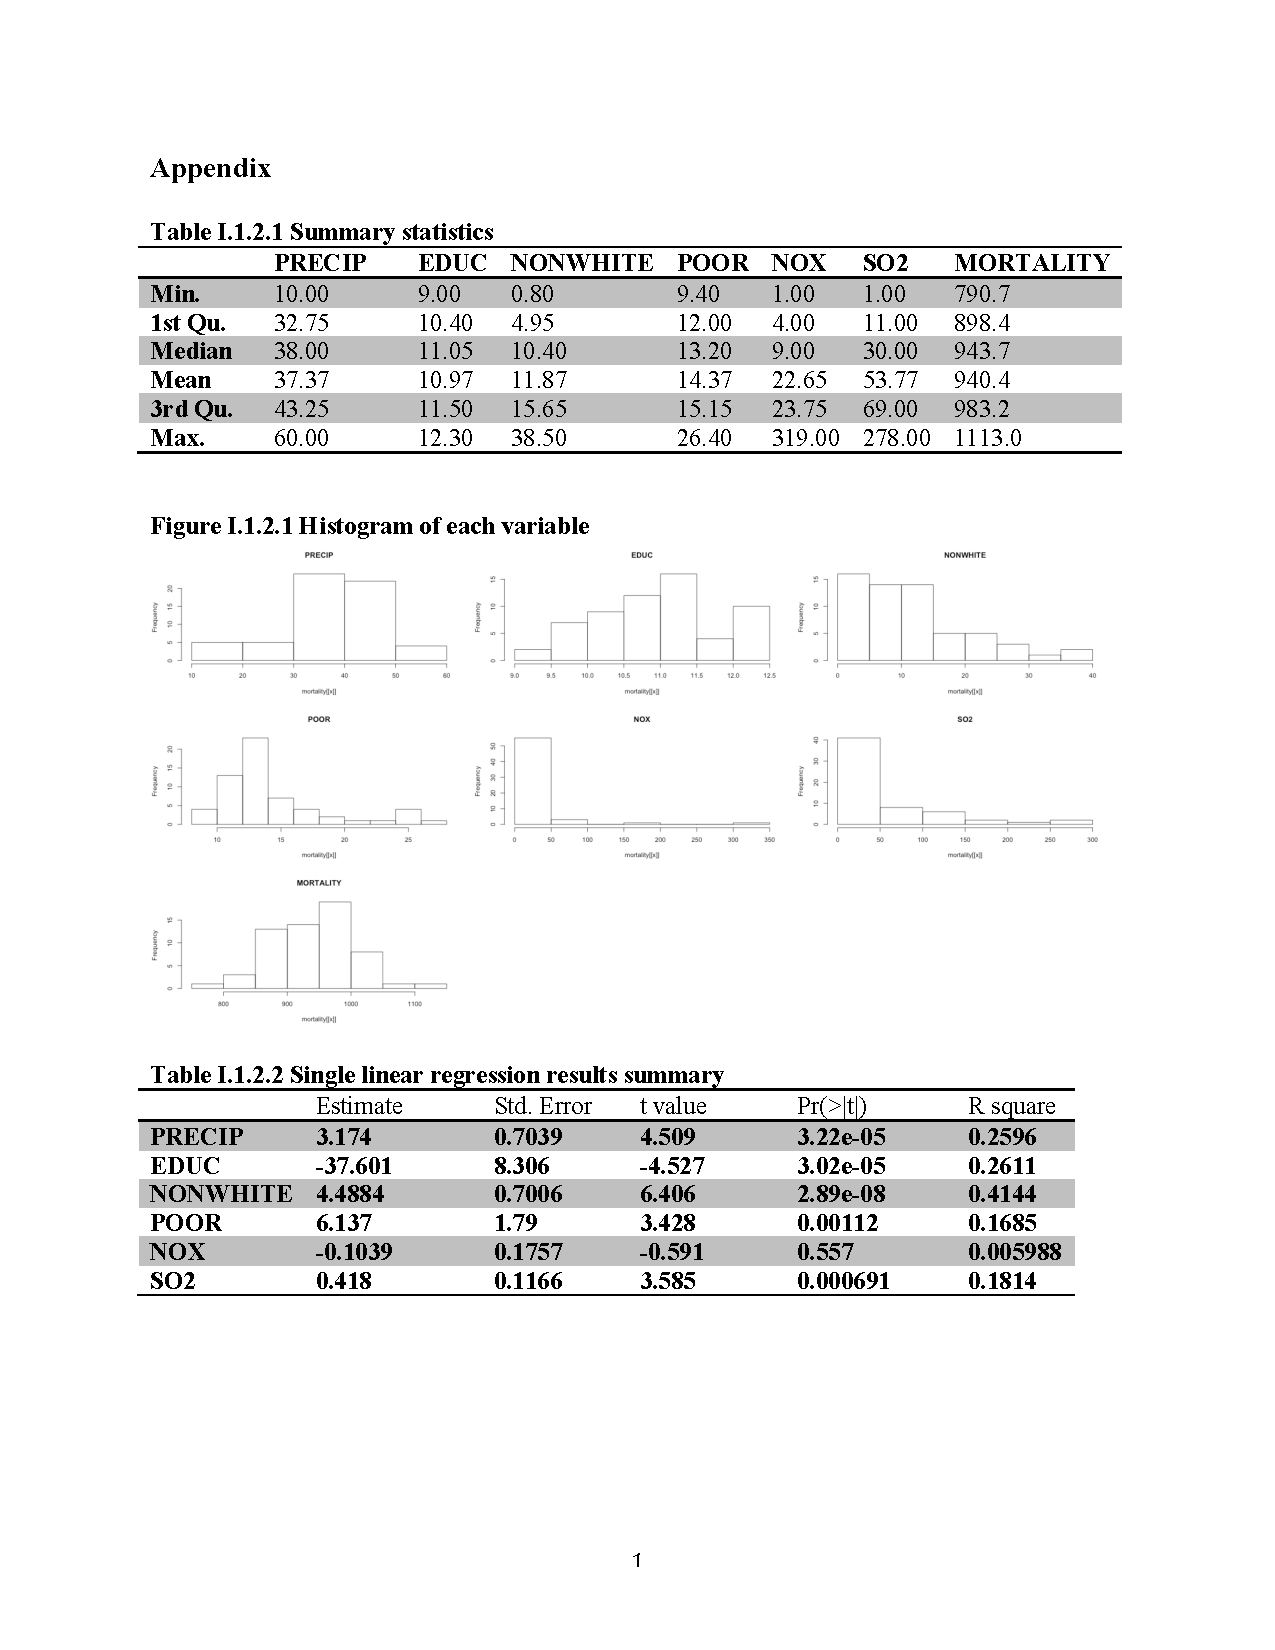
\includepdf[pages=-]{appendix.pdf}

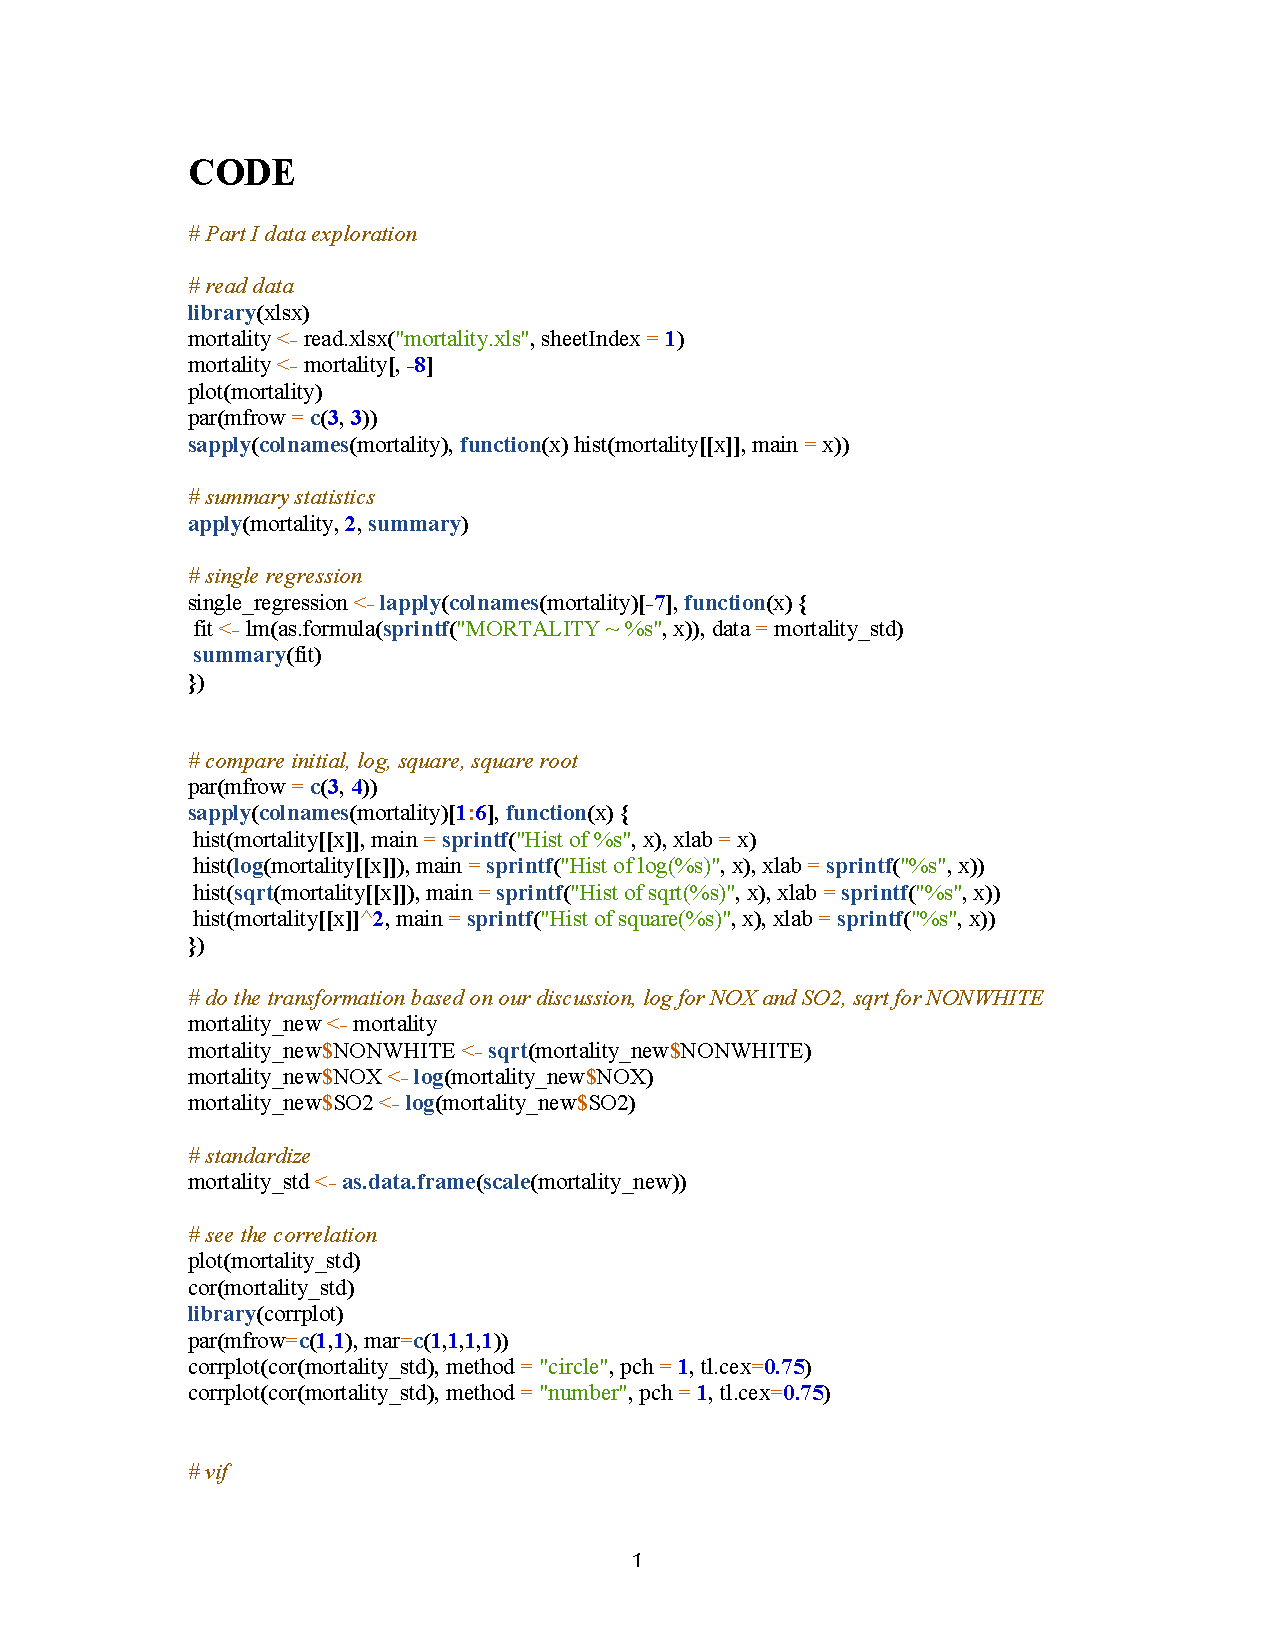
\includepdf[pages=-]{STA207_project_code.pdf}

\end{document}
